\section{Test Function Documentation}
To be able to make easy and similar test' for all the layers, it was decided that we developed a function to make test. The function is able to send data to a layer as if it was theneighbour layers. Thus the function makes it possible to give input to a layer and check the output.

\begin{figure}[htb]
	\begin{center}
	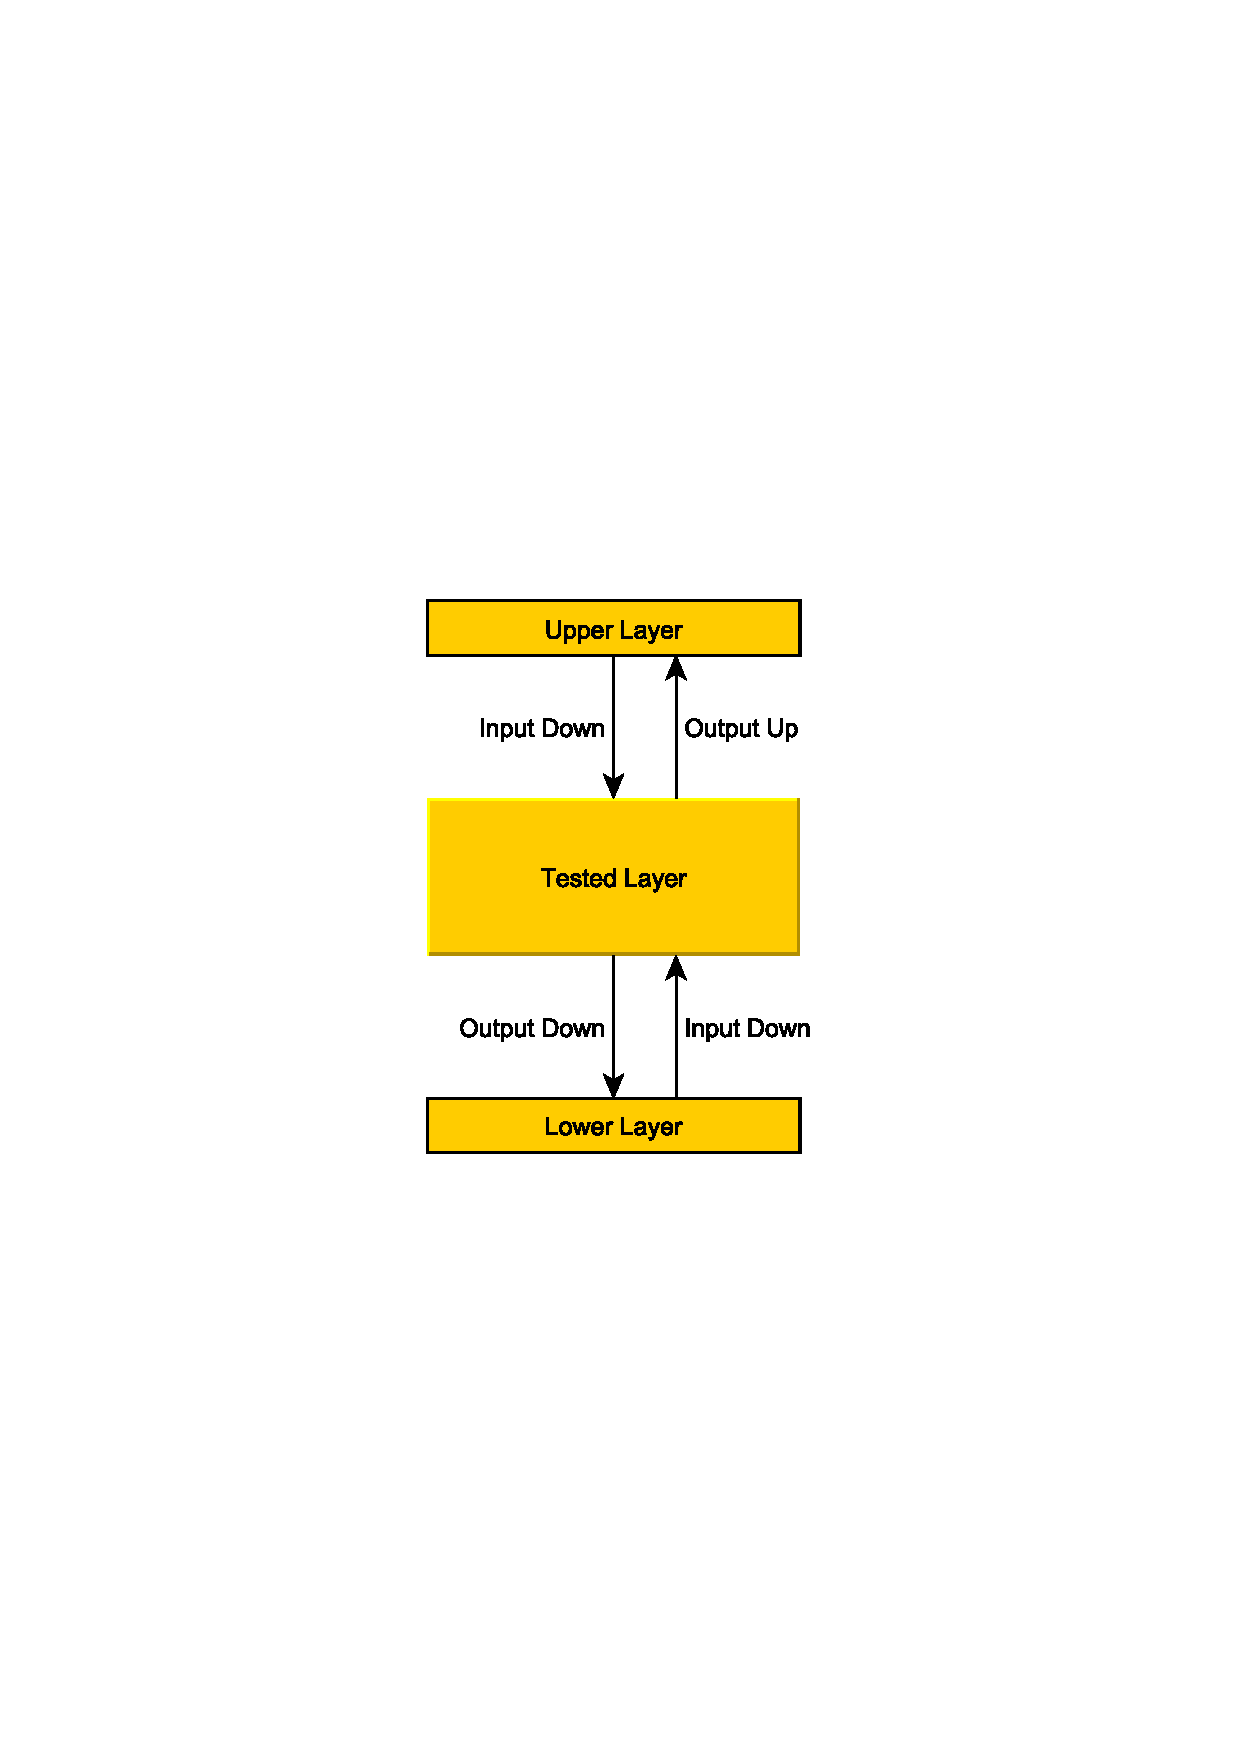
\includegraphics[scale=0.5,trim=0 0 0 0]{Layer_inputoutput.pdf}
	\caption{Substituting surrounding layers (incomplete)}
	\label{fig:Layer_inputoutput}	
	\end{center}
\end{figure}

Use of Input Output functions
To make it easy to change and manipulate the input and output, is it defined in .dat documents. Therefore the program doesn?t have to be changed for different input, and the output can be easily extracted for further analysis. Ifstream and Ofstream are used to read and write from the documents. In the 
BOOST buffer
As the boost buffer is used as communication between the layers, is it also used as the test functions mean of communication with the layer tested. There are defined four buffers, two for input and two for output.
Use of test function
In the beginning one simply includes the layer and in the function sets the name of the layer. It?s is possible to change the defined names for the .dat files. The boost buffers are defined for the layer, so with this setup it?s just running the program.

\begin{figure}[htb]
	\begin{center}
	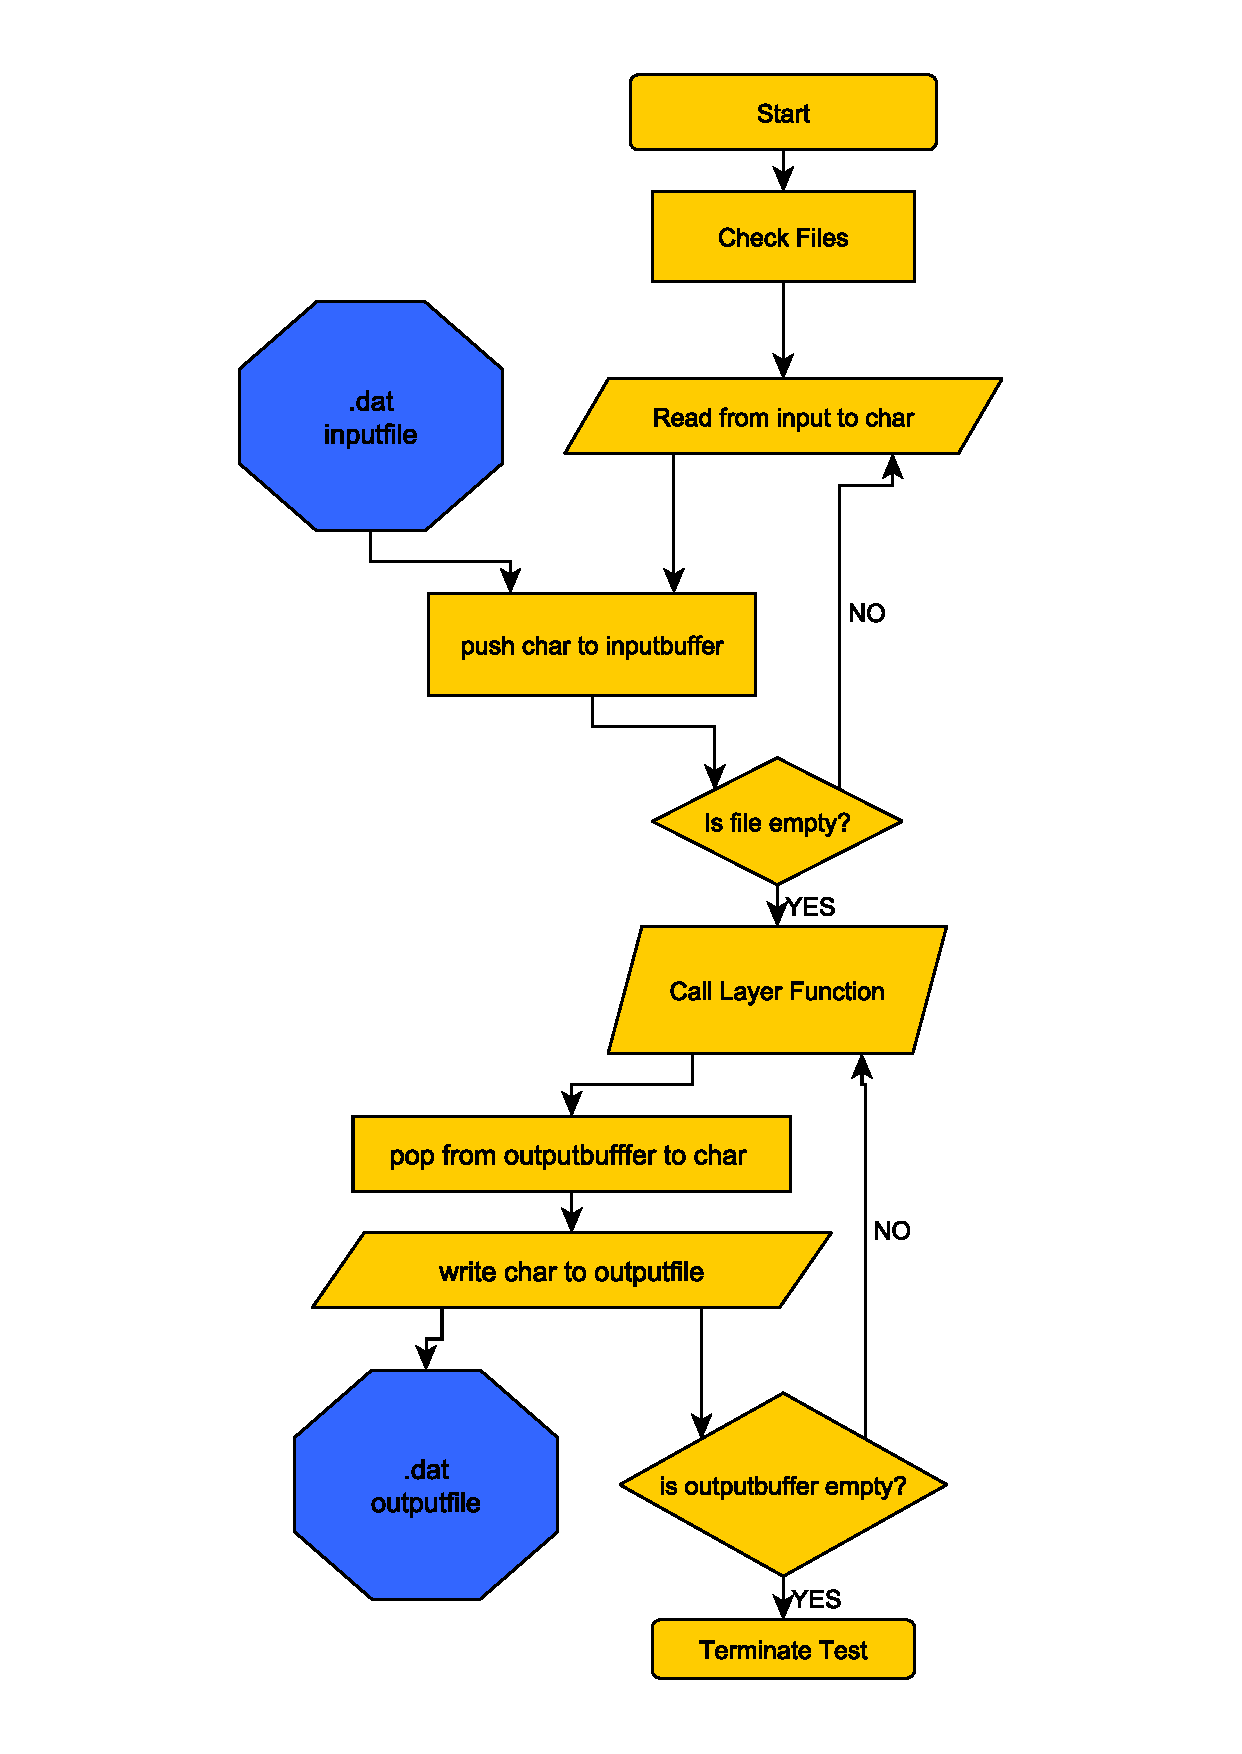
\includegraphics[scale=0.5,trim=0 0 0 0]{TestFlowchart.pdf}
	\caption{Flowchart for test function (incomplete)}
	\label{fig:TestFlowchart}	
	\end{center}
\end{figure}

